\section{Results}
\label{sec:results}

We used our software to perform various \acrshort{wpd} simulations.
In this section we present the results of some of these simulations.
We will shortly introduce the simulated scenarios.
We also want to provide some formulas to analytically validate the correctness of some of the simpler scenarios.
Our simulator uses the Hartree atomic units \cite{hartree_1928}.
Every quantity in the upcoming part should be interpreted as such.
You can find animations showing the time evolution of \acrshort{wp}s on  \url{https://zoltansimon.info/src/content/research/wavepacketsim.html}.

First we would like to present the simulation results of an electron diffraction experiment.
Many different forms of diffraction can be explained using \acrshort{qm}.
The scale at which diffraction happens ranges from the scale of subatomic particles  to larger molecules.
Measuring diffraction patterns is a very useful tool in the hand of scientists.
It provides information about the object that caused the diffraction.
At this point it is probably important to emphasize that the diffraction of light is a different phenomenon since light is an electromagnetic wave.
Whit that said, the fact that particles are not electromagnetic waves but still exhibit wave-like behavior as discussed is section \ref{sec:theory} makes this experiment even more interesting.
Diffraction of a particle happens when the \acrshort{wp} of the particle passes through some kind of a barrier.
In our simulation we can model the barrier as a specifically initialized localized potential.
The \acrshort{wp} arrives from one side of the barrier.
While passing through this barrier it diffracts and some of the \acrshort{wp} gets reflected back.
The portion of the \acrshort{wp} that passed through --suffering diffraction-- continues forward and consequently arrives to a measuring device.
In our simulation our measuring device is a virtual canvas where we measure the probability density.
A simple diffraction scenario is the double-slit experiment.
Here the barrier is a potential wall with two narrow parallel slits.
The \acrshort{wp} passes through these slits.
According to the Huygens–Fresnel principle in diffraction experiments we can approximate the wave function after the barrier as concentric waves emitted from the slits or holes of the barrier.
This gives a simple enough model to predict the shape of interference pattern forming on the canvas.
We would like to validate the distance between the stripes in the interference pattern.
To calculate the distance between the probability density peaks first we have to get a formula for the intensity on the canvas.
\begin{equation}
	\label{eq:Huygens}
	I(\vec{r}) = I_0 \frac{sin^2\left( \pi N \frac{dy}{\lambda L} \right)}{sin^2\left( \pi \frac{dy}{\lambda L} \right)}
\end{equation}
where $N$ is the number of holes on the barrier (in double-slit experiment $2$), $d$ is the distance between the holes, $L$ is the distance between the canvas and the barrier $\lambda$ is the wavelength of the wave and $y$ is the location on the canvas.
We performed the simulation using $L = 30$ Bohr radii, $d = 2.5$ Bohr radii, $\lambda = \frac{2\pi}{3}\simeq 2.1$ Bohr radii with two slits.
The width of each slit was a small enough value of $0.5$ Bohr radii.
\begin{figure}
	\begin{center}
		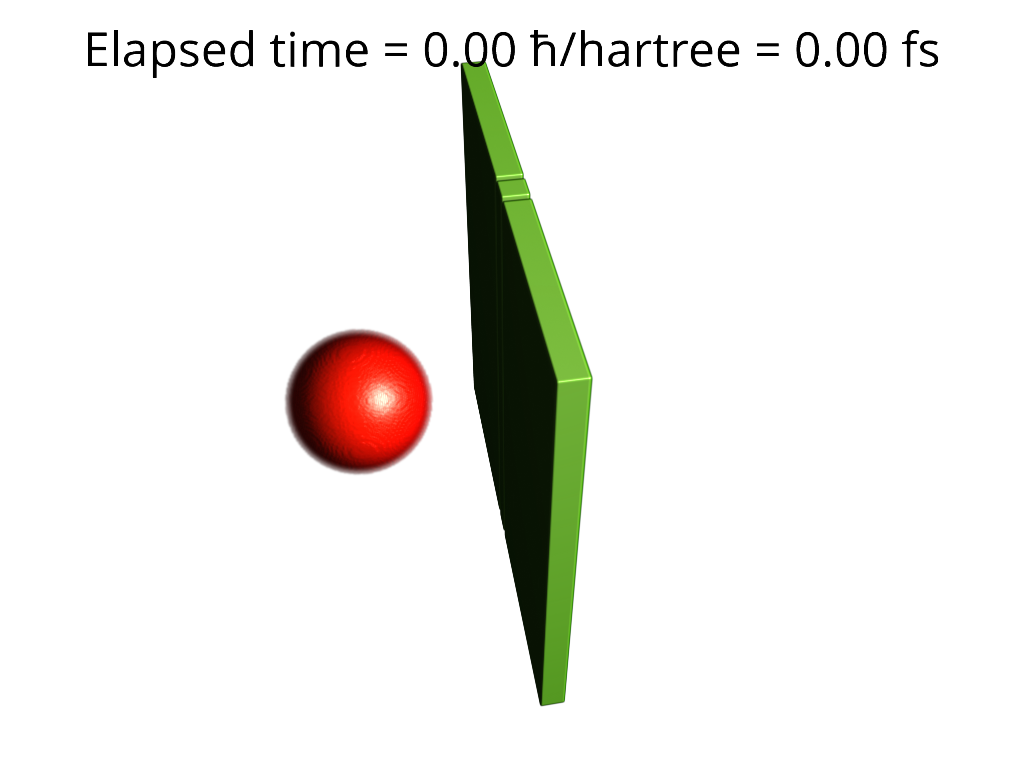
\includegraphics[width=0.32\textwidth]{figures/double_slit_01.png}
		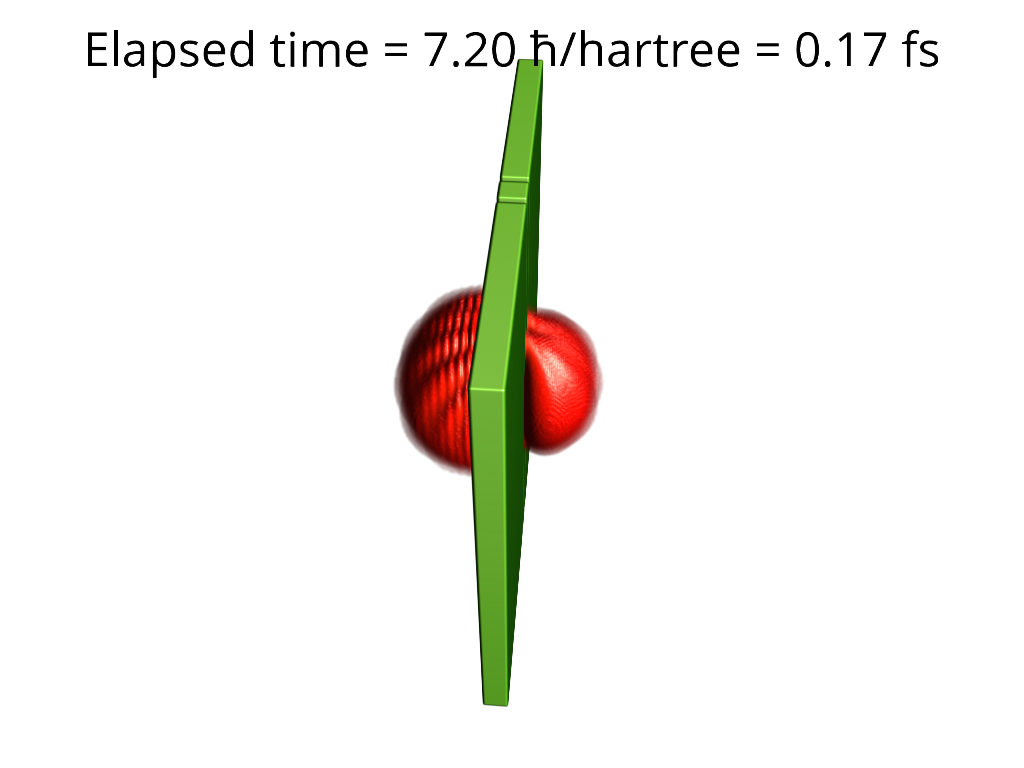
\includegraphics[width=0.32\textwidth]{figures/double_slit_02.png}
		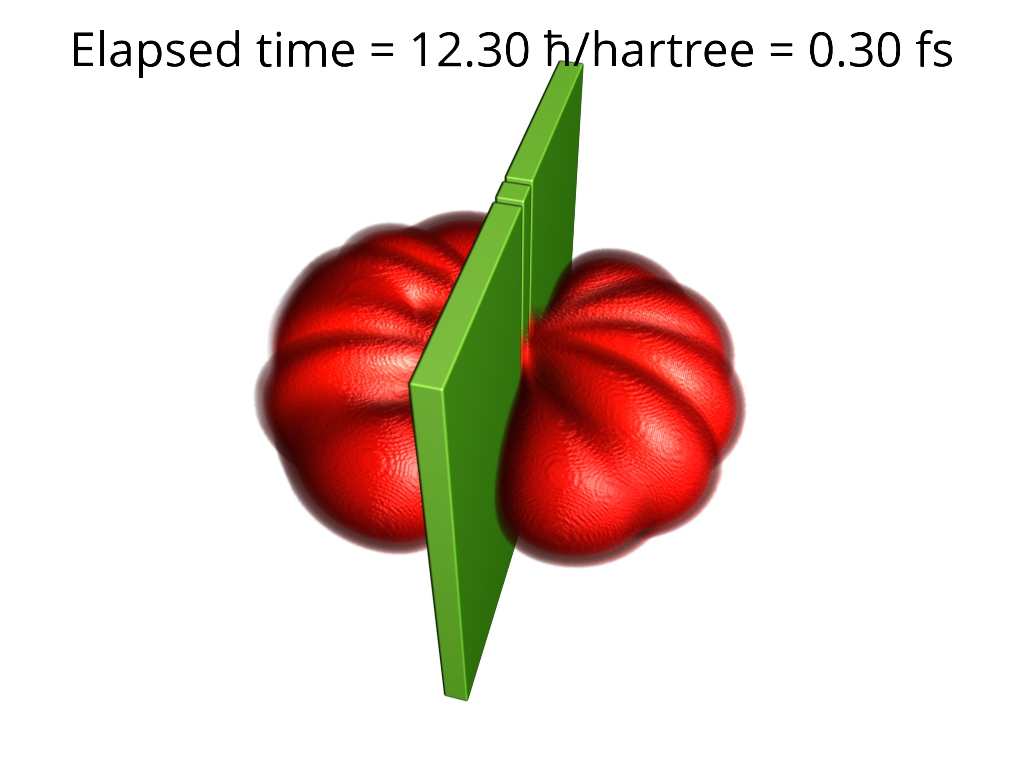
\includegraphics[width=0.32\textwidth]{figures/double_slit_03.png}
		\caption{Stages of the double-slit experiment: before, during and after passing through the double-slit}
		\label{fig:double_slit_stages}
	\end{center}
\end{figure}
Different stages of double-slit simulation can be seen in figure \ref{fig:double_slit_stages} where we have used ray tracing to visualize the probability density and the potential.
The interference pattern is visualized in figure \ref{fig:double_slit_interference} on a canvas of size $60 \times 60$ Bohr radius.
We compared the simulated pattern and the pattern predicted by the Huygens–Fresnel principle.
It can be seen that that the two patterns are very similar.
\begin{figure}
	\begin{center}
		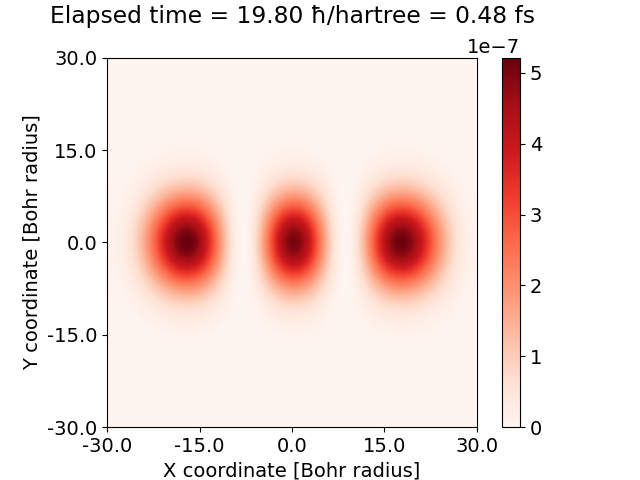
\includegraphics[width=0.5\textwidth]{figures/double_slit_interference.png}
		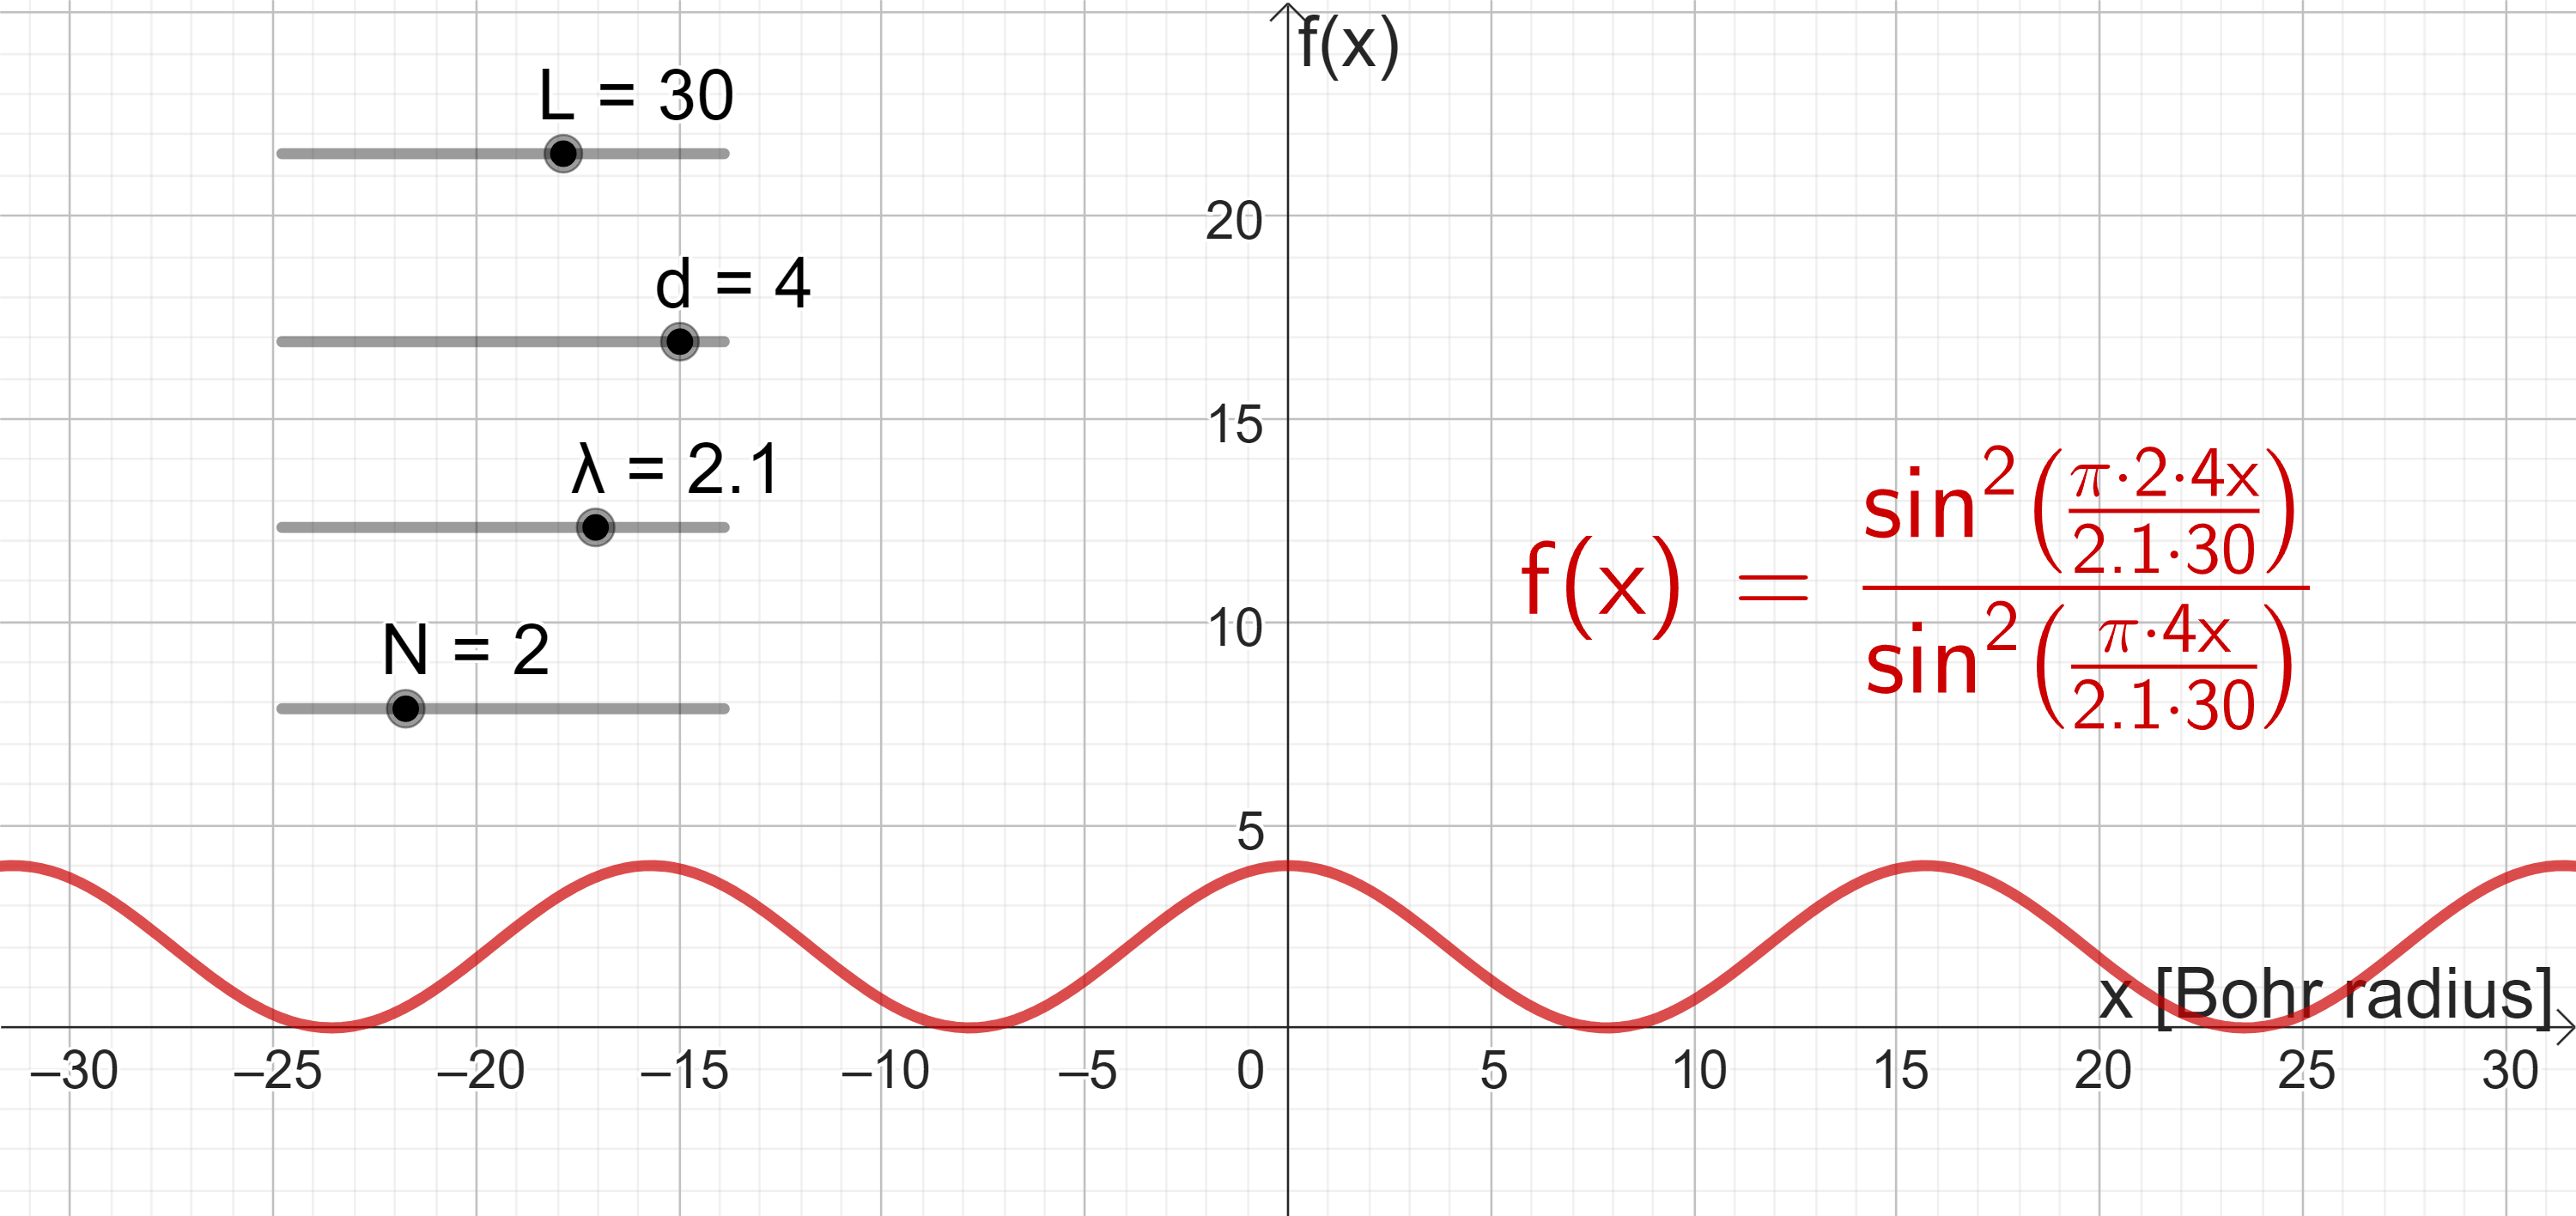
\includegraphics[width=0.5\textwidth]{figures/validation_of_double_slit.png}
		\caption{Comparison of the simulated (above) and the analytically predicted (below) interference pattern during double-slit experiment}
		\label{fig:double_slit_interference}
	\end{center}
\end{figure}


Note that in equation \ref{eq:Huygens} $y$ is a one dimensional coordinate. Indeed the double-slit experiment can be fully described using only two spatial dimensions and the diffraction pattern forms in a single dimension perpendicular to the propagation direction of the wave.
The make use of all three simulated dimensions we also recreated diffraction on optical grid.
An optical grid is a structure of multiple potential nodes arranged in a pattern.
The holes between the potential nodes behave like the holes in the previous experiment.
We put 11 nodes in each direction forming a rectangular grid.
Each node has a Gaussian potential distribution and a maximal potential of $8$ hartree.
The distance between adjacent grid points is $d = 4$ Bohr radii.
The canvas distance is $L=30$ Bohr radii and the wavelength is $\lambda\simeq 2.1$ Bohr radii as in the previous simulation.
In figure \ref{fig:optical_grid_stages} we visualized different stages of the time development using ray tracing.
\begin{figure}
	\begin{center}
		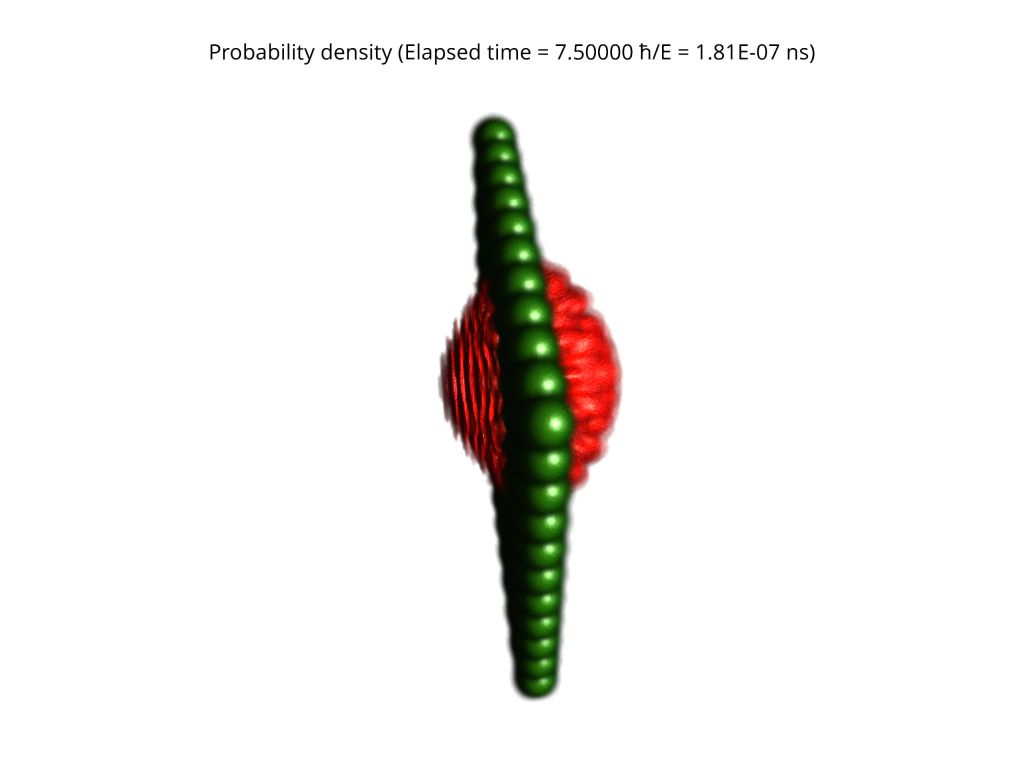
\includegraphics[width=0.32\textwidth]{figures/optical_grid_01.png}
		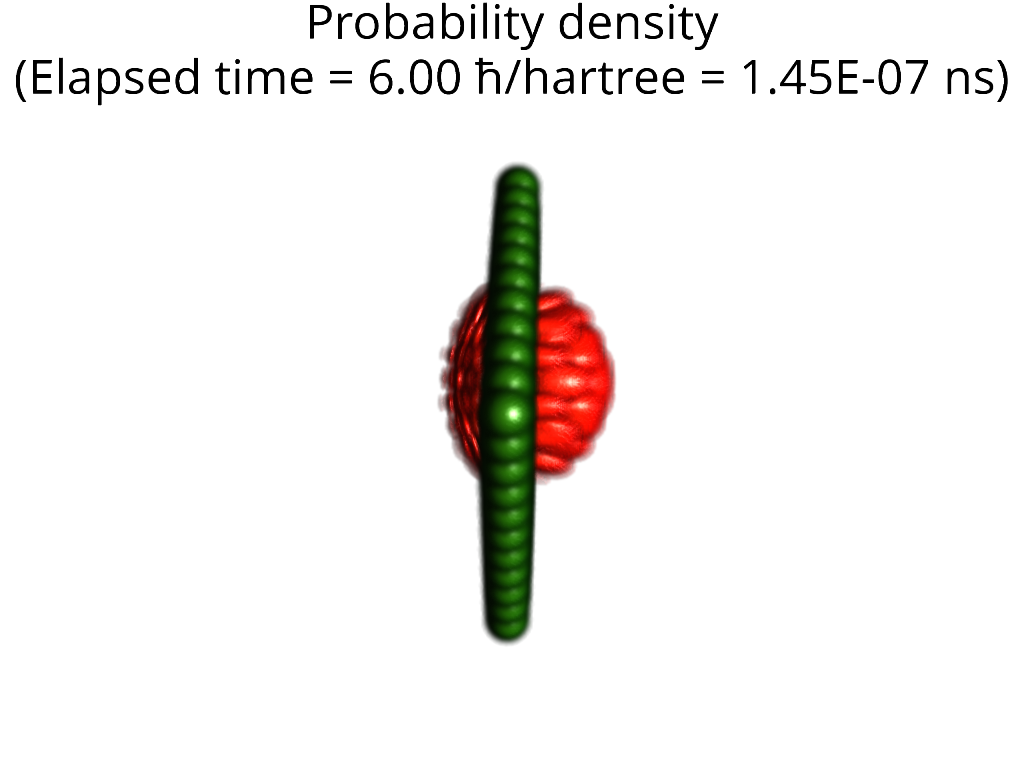
\includegraphics[width=0.32\textwidth]{figures/optical_grid_02.png}
		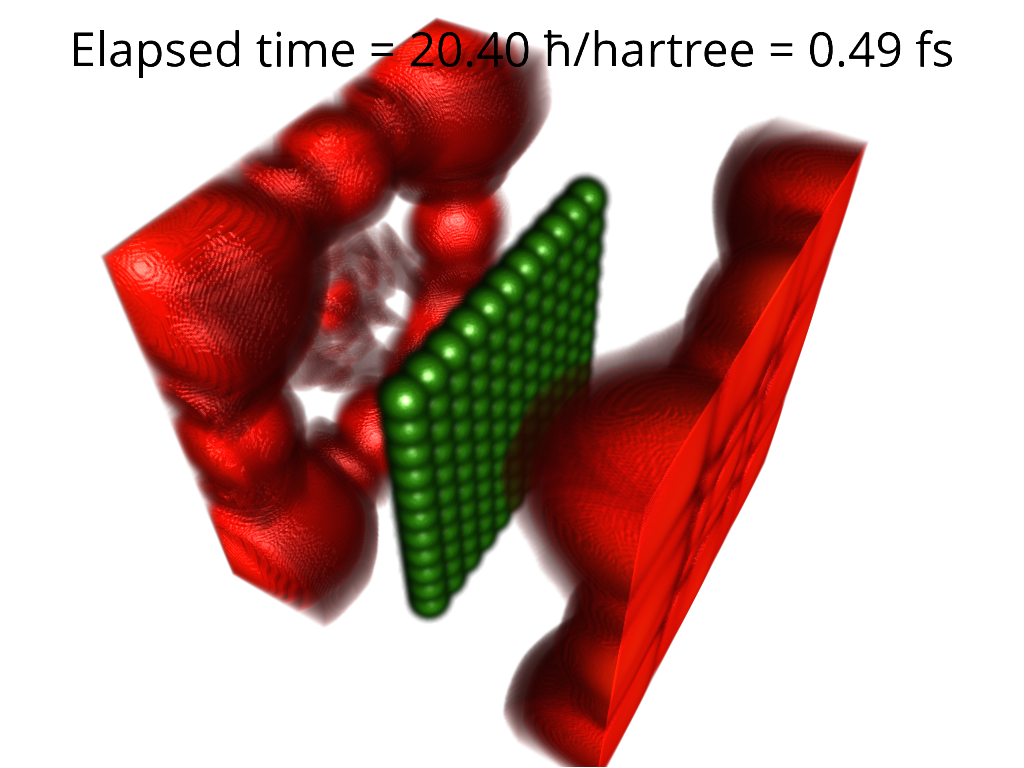
\includegraphics[width=0.32\textwidth]{figures/optical_grid_03.png}
		\caption{Stages of the optical grid experiment: during, right after and later after passing through the grid}
		\label{fig:optical_grid_stages}
	\end{center}	
\end{figure}
During the simulation many interesting interference patterns arise.
We showcase some of these in figure \ref{fig:optical_grid_interference}.
\begin{figure}
	\begin{center}
		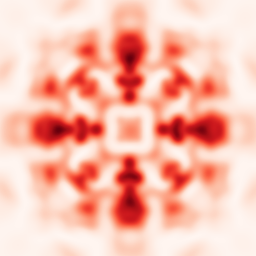
\includegraphics[width=0.32\textwidth]{figures/optical_grid_interference_01.png}
		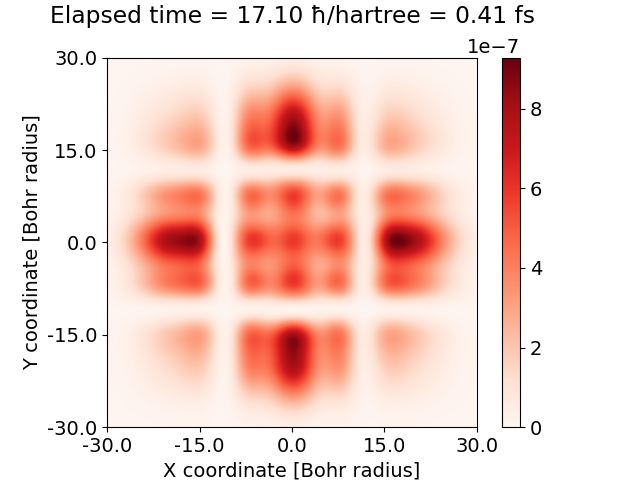
\includegraphics[width=0.32\textwidth]{figures/optical_grid_interference_02.png}
		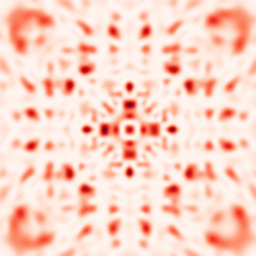
\includegraphics[width=0.32\textwidth]{figures/optical_grid_interference_03.png}
		\caption{Three stages of interference patterns forming on the measurement canvas during optical grid simulation}
		\label{fig:optical_grid_interference}
	\end{center}	
\end{figure}

One interesting use case of a higher dimensional \acrshort{wpd} simulator is that the higher dimensional space can be used to model the interactions between multiple lower dimensional particles.
For example our 3D simulation is capable of the simulation of three 1D particles.
To do this we have to define special interaction potential.
To create such potential we have to think about the coordinates in the higher dimensional configuration space as the coordinates of the lower dimensional space describing the location of the lower dimensional particle.
If the potential potential energy affecting all particles can be expressed as a $V(x_a, x_b, x_c)$ function of the location of particle $A$ and $B$ and $C$ than we can reinterpret this function as the $V(\vec{r})$ localized potential function used in the potential propagator in equation \ref{eq:potential_prop}.
Note that here $\vec{r}$ becomes $(x_a, x_b, x_c)$.
To model the interaction between the three 1D particles we initialized a linear combination of two types of interaction potentials.
One is proportional to $\frac{1}{|x_i - x_j|}$ where $i,j\in\{a,b,c\}$ and $i\neq j$ and the other is a hard interaction that takes it's maximum if the particles approach each other inside an $\epsilon$ radius otherwise it's zero.
To prevent blotting of the Gaussian \acrshort{wp} we also initialized a harmonic oscillator potential.
This helps because the Gaussian $wp$ is the eigenstate of the harmonic oscillator.
The potential for a harmonic oscillator is given in the following form
\begin{equation}
	\label{eq:harmonic_osc}
	V(x) = \frac{m\omega^2}{2}x^2
\end{equation}
where $m$ is the oscillating weight and $\omega$ is the angular velocity of the oscillation.
First we created a scenario where particle $A$ starts at $25$ Bohr radii away from to center of the oscillator where the potential energy is maximal thus it accelerates towards the other two particle consequently transferring the momentum to the particle on the far right.
For this experiment the interaction potential consists only from the hard interaction.
The angular velocity of the oscillator is $\omega = \frac{2\pi}{44} \simeq 0.1415\; \frac{rad\cdot hartree}{\hbar}$.
After the collision particle $C$ propagates towards the maximal potential of the oscillator.
Particle $B$ stays in place since it served only as a medium in the momentum transfer.
The momentum gained from particle $A$ was immediately given to particle $C$.
When all of it's kinetic energy is transferred to potential energy than it turns back.
The oscillation with the momentum transfer between the particles continues.
Different phases of this simulation can be observed on the per axis visualization in figure \ref{fig:1d_particles_in_oscillator_stages}.
\begin{figure}
	\begin{center}
		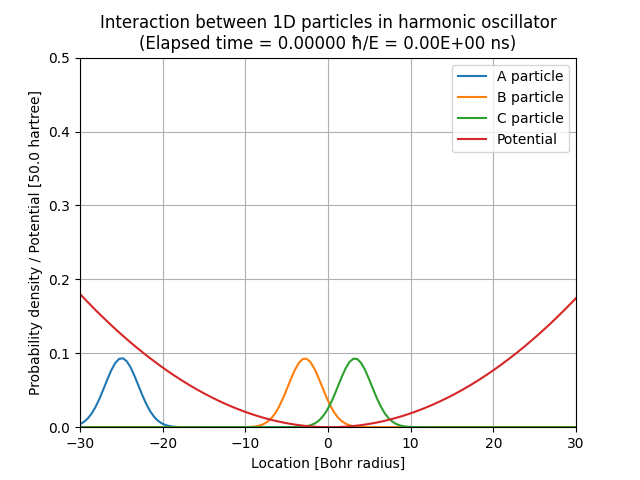
\includegraphics[width=0.32\textwidth]{figures/1d_oscillator_01.png}
		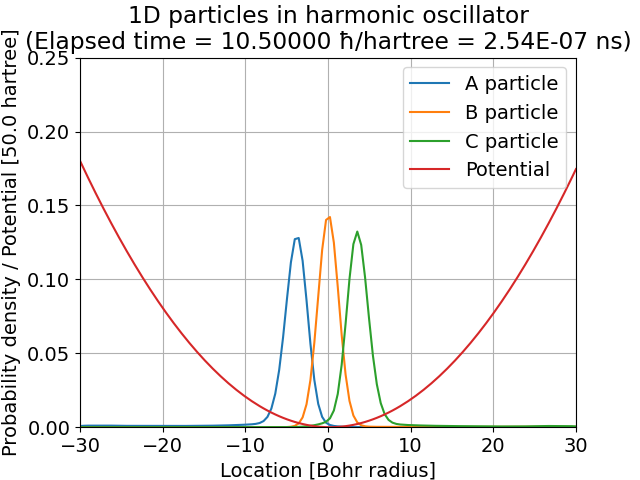
\includegraphics[width=0.32\textwidth]{figures/1d_oscillator_02.png}
		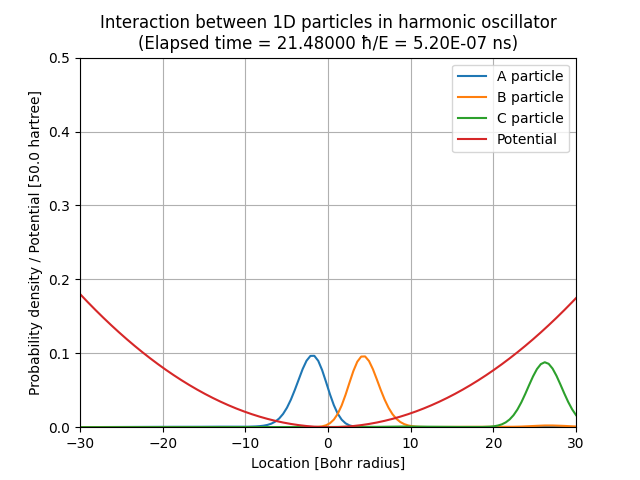
\includegraphics[width=0.32\textwidth]{figures/1d_oscillator_03.png}
		\caption{Stages of the interactions between 1D particles in harmonic oscillator: initial state, particle A giving momentum to particle C, particle C reaching maximal potential and turning back}
		\label{fig:1d_particles_in_oscillator_stages}
	\end{center}
\end{figure}
Please note that particle $C$ converts all of it's kinetic energy to potential energy right at the half of the first period of the oscillation $t = 44 / 2 \frac{\hbar}{hartree} \simeq 21,48 \frac{\hbar}{hartree}$.
This means that the harmonic oscillator functions correctly.

Now let's repeat the this experiment but now we place a finite potential barrier in the middle of the oscillator.
The probability of a particle with $E$ energy tunneling through a $d$ thick barrier of $V_0$ potential can be expressed in the following form
\begin{equation}
	\label{eq:tunelling probability}
	\probP_{tunnel} = \frac{1}{1 + \frac{V_0^2}{4E(V_0 - E)}sinh^2(\kappa d)}
\end{equation}
where $\kappa = \sqrt{2m(V_0 - E)}\;/\hbar$ is determined by the energy of the incoming \acrshort{wp}.
Energy is conserved so $E = V(x_A)$.
We solve for $\probP_{tunnel} = \frac{1}{2}$.
One possible solution is $V_0 \simeq 8.5$ hartree and $d \simeq 0.3$ Bohr radius.
Particle $A$ gives it's momentum to $B$ as before.
With these parameters approximately the half of the probability density of particle $B$ tunnels through the barrier giving it's momentum to particle $B$ on the next side of the wall.
This causes the $C$ to start moving with probability of approximately $\frac{1}{2}$.
This can be observed in figure \ref{fig:1d_osc_with_tunneling}.
\begin{figure}
	\begin{center}
		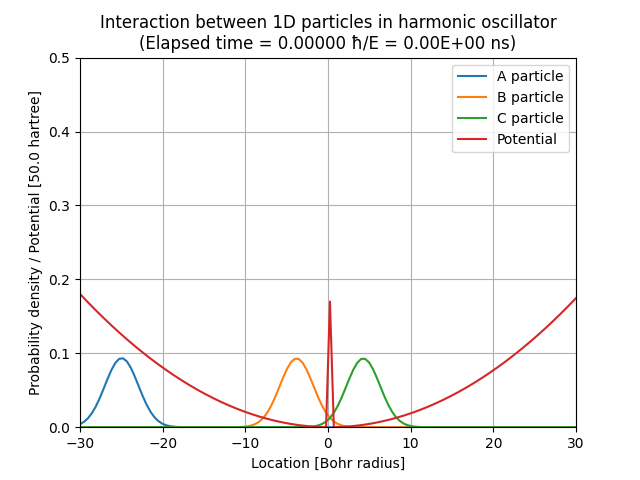
\includegraphics[width=0.32\textwidth]{figures/1d_oscillator_tunneling_01.png}
		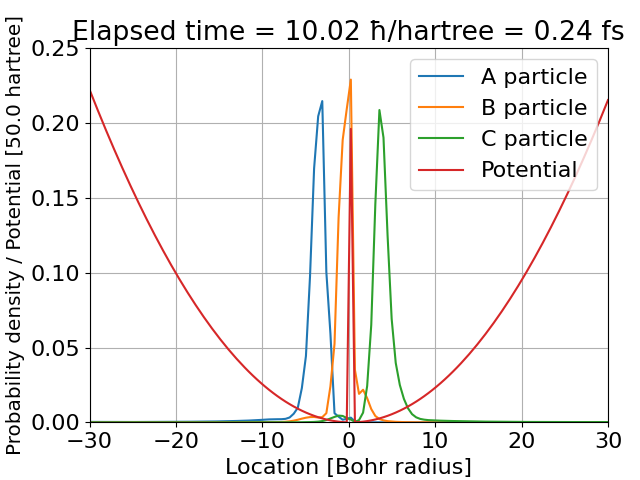
\includegraphics[width=0.32\textwidth]{figures/1d_oscillator_tunneling_02.png}
		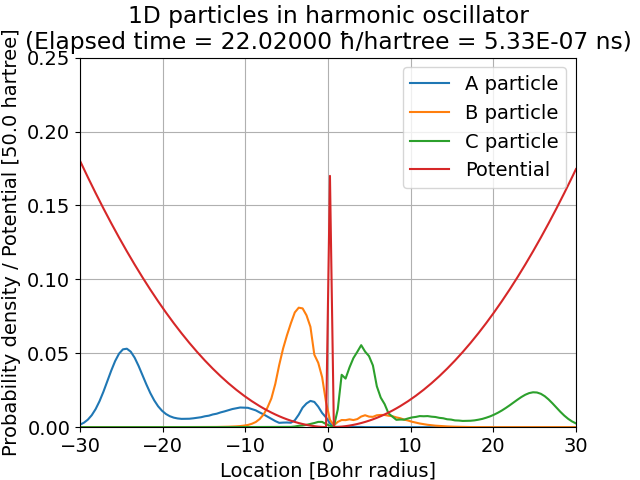
\includegraphics[width=0.32\textwidth]{figures/1d_oscillator_tunneling_03.png}
		\caption{Stages of the interactions between 1D particles in harmonic oscillator: initial state, particle A giving momentum to particle C, particle C reaching maximal potential and turning back}
		\label{fig:1d_osc_with_tunneling}
	\end{center}	
\end{figure}

Our last group of simulations try to model the working of a flash memory cell.
The flash memory is used extensively in many modern electronic devices such as smart phones, laptops or tablets.
The general structure of a cell is visualized in figure \ref{fig:flash_memory}.
A flash memory stores information by trapping electrons on a floating gate.
The writing and flushing of the a flash cell is performed by inducing a strong enough electric field that the electron can tunnel through the potential barrier between the floating gate and the channel.
The reading of a memory cell is done by inducing current through the the channel between the source and the drain.
If there are electrons trapped on the floating gate they create a Coulomb potential shifting the potential in the substrate allowing or denying the flow of electrons between the drain and the source thus the resistance changes and the information about the state of the floating gate was successfully retrieved.
\begin{figure}
	\centering
	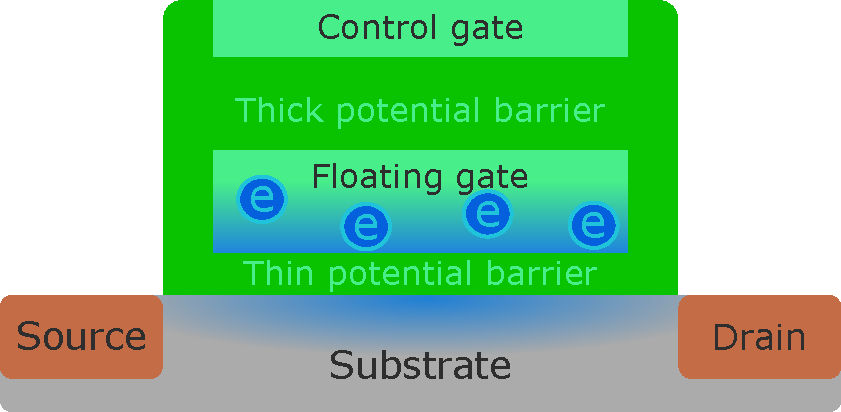
\includegraphics[width=0.5\textwidth]{figures/flash_memory.pdf}
	\caption{Structure of a flash memory cell}
	\label{fig:flash_memory}
\end{figure}
In figure \ref{fig:flash_memory} we used brighter green for the potential barriers.
It can be seen that between the control gate and the floating gate there is a thicker potential barrier.
This prevents the flow of electrons between these two parts.
Only the Coulomb potential induced by the electrons on the control gate must be felt by the electrons on the floating gate.
In order to the writing and flushing to be possible the thickness and height of the potential wall between the floating gate and the substrate must be chosen carefully.
This barrier must be thick enough to prevent unwanted tunneling when the control gate is empty.
After the control gate fills with electrons the Coulomb potential created by those electrons makes an overall slope in the potential.
This slope adds to the potential wall thus changing its shape.
The previously rectangular barrier now acquired a triangular outline. More importantly the $d$ length of the barrier gets reduced.
This increases the probability of the electron in floating gate to tunnel out from the gate. This is sound with equation \ref{eq:tunelling probability} for the probability of tunneling.
This is phenomena is called Fowler–Nordheim tunneling \cite{Fowler_1928bv}.
In our first flash memory related simulation we have initialized a wall that represents the barrier between the floating gate and the substrate.
Our simulation deals with only one electron.
This initialize the location of this electron to be inside the floating gate.
When we want to simulate the flushing of the cell, we add a Coulomb potential the decreases towards the barrier.
Create initialized the barrier to have a height of $V_0 = 10$ hartree and width of $d = 1.0$ Bohr radius.
From the other sides we fully enclosed the floating gate with thicker potential barriers the so that the electron can only tunnel through the desired barrier.
We gave an initial momentum to our \acrshort{wp} towards the barrier.
We initialized the Coulomb potential to have take it's maximal value on the control gate and so that it gives a 50.
We run the simulation with the Coulomb potential turned on and off and compared the probability evolution plots.
Figure \ref{fig:flash_flush_plot} shows the flushing of the floating gate with the Coulomb potential enabled.
The probability of the electron being found on the gate is rapidly decreasing.
\begin{figure}
	\centering
	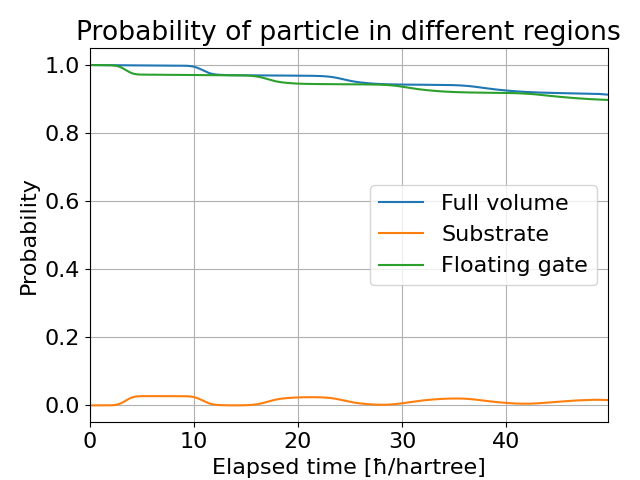
\includegraphics[width=0.5\textwidth]{figures/flash_flush.png}
	\caption{Flushing of the floating gate}
	\label{fig:flash_flush_plot}
\end{figure}
In figure \ref{fig:flash_keep} however the the electron stays much longer on the gate since here we disabled the potential slope.
This shows that by by changing the electric field we can control the writing and flushing of the floating gate.
\begin{figure}
	\centering
	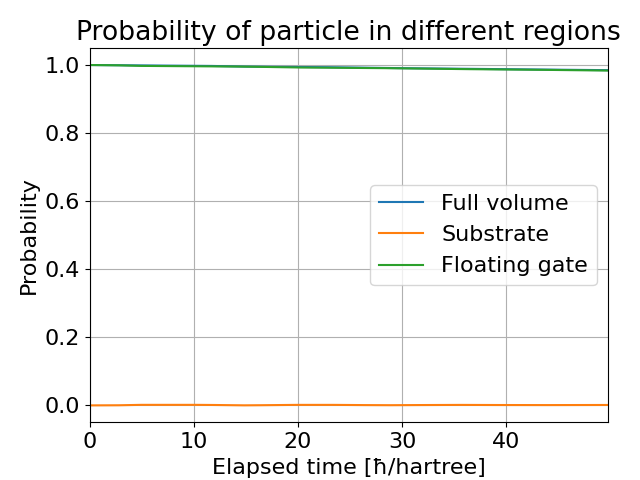
\includegraphics[width=0.5\textwidth]{figures/flash_keep.png}
	\caption{Storing the electron on the floating gate over a longer period of time}
	\label{fig:flash_keep}
\end{figure}






